\documentclass[conference, draftcls,12pt]{IEEEtran}

%\usepackage{amsmath}
\usepackage{booktabs} % For formal tables

\usepackage{cite}
\usepackage{standalone}

\usepackage{listings}
\lstset{ %
    basicstyle=\footnotesize\ttfamily,
}

\usepackage{graphicx}
\usepackage{hyperref}
\usepackage{cleveref}

\usepackage{lipsum}

\begin{document}
\title{Porto Seguro's Safe Driver Prediction\\Project Status Report}
\author{
\IEEEauthorblockN{Hanlin He, Mingze Xu, Su Yang, Tao Wang}
\IEEEauthorblockA{Department of Computer Science, The Erik Jonsson School of Engineering and Computer Science\\
The University of Texas at Dallas\\
Email:
\{hxh160630, mxx160530, sxy161730, txw162630\}@utdallas.edu}}

\maketitle

\begin{abstract}
This is the project status report of Porto Seguro's Safe Driver Prediction. Some of the content would be part of the final report.
\end{abstract}

\documentclass{standalone}

\begin{document}

\section{Introduction}

Machine learning is emerging in the insurance industry and is being applied
across multiple areas including the interpretation of data, business operations
and driver safety. One key application is claim prediction. Inaccuracies in car
insurance company's claim predictions raise the cost of insurance for good
drivers and reduce the price for bad ones. A more accurate prediction will
allow insurers to further tailor their prices, and hopefully make auto
insurance coverage more accessible to more drivers.

In this report, we based on Kaggle's Featured Prediction Competition
\emph{Porto Seguro's Safe Driver Prediction}\cite{kaggle}, conducted several
experiments, compared different approaches' effectiveness to tackle the claim
prediction problem, including \emph{logistic regression}, \emph{random forest}
and \emph{gradient boosting}.

The organization of the following report is as follows. In \cref{problem}, we
will formally define the problem to solve and discuss the theoretical principle
of the algorithm we used. Then we will analyze the data feature and our method
of feature engineering in \cref{preprocessing}. After that, the experimental
results are shown and analyzed in \cref{evam}. Finally, we will discuss related
works in \cref{related} and conclude the report in \cref{conclusion}.

\end{document}


\documentclass{standalone}

\begin{document}

\section{Problem Definition and Algorithm}\label{problem}

\subsection{Task Definition}

%Precisely define the problem you are addressing (i.e. formally specify the
%inputs and outputs). Elaborate on why this is an interesting and important
%problem. 

A machine learning problem is defined as to learn from experience $E$ with
respect to some class of tasks $T$ and performance measure $P$, if its
performance at tasks in $T$, as measured by $P$, improves with experience
$E$\cite{Mitchell:1997:ML:541177}.
The claim prediction problem can be defined as follow:
\begin{itemize}[\IEEEsetlabelwidth{Z}] 
    \item[$E$] previous year's policy holders' information and whether or not a
        claim was filed for that policy holder.
    \item[$T$] predicting the possibility that an auto insurance policy
        holder will file an insurance claim next year.
    \item[$P$] the accuracies and Gini Coefficient was used to measure the
        effectiveness of models.
\end{itemize}

\subsection{Algorithm Definition}

We used logistic regression, ensemble methods like random forests and gradient boost in our model building. In this
section, we will discuss the theoretical foundation of these algorithms.

\subsubsection{Logistic Regression}

Logistic Regression is an approach to learning functions of the form $f:X\rightarrow Y$\cite{Mitchell:2016} or in our case $P(Y|X)$ where $Y$ is discrete-valued, and $X = \langle X_1 ...X_n\rangle$ is any vector containing discrete and continuous variables. The parametric model assumed by Logistic Regression in the case where Y is Boolean is:
\begin{IEEEeqnarray}{Rl} 
P(Y=1|X)&=\frac{1}{1+\exp(w_0+\sum_{i=1}^nw_iX_i)}\IEEEnonumber\\
P(Y=0|X)&=\frac{\exp(w_0+\sum_{i=1}^nw_iX_i)}{1+\exp(w_0+\sum_{i=1}^nw_iX_i)}\IEEEnonumber
\end{IEEEeqnarray}

One reasonable approach to training Logistic Regression is to choose parameter values that maximize the conditional data likelihood. We also used regularization to reduce the overfitting problem. The penalized log likelihood function is as followed:
\begin{IEEEeqnarray}{C} 
W \leftarrow \arg\max_W\sum_l\ln{P(Y^l|X^l,W)}-\frac{\lambda}{2}||W||^2\IEEEnonumber
\end{IEEEeqnarray}
where the last term is a penalty proportional to the squared magnitude of $W$.

In general, the algorithm used gradient ascent to repeatedly update the weights in the direction of the gradient, on each iteration changing every weight $w_i$, beginning with initial weights of zero, according to:
\begin{IEEEeqnarray}{C} 
w_i \leftarrow w_i+\eta\sum_lX_i^l(Y^l-\hat{P}(Y^l=1|X^l,W))-\eta\lambda{w_i}\IEEEnonumber
\end{IEEEeqnarray}
where $\eta$ is a small constant which determines the step size.

The actual implementation of Scikit-learn library includes multiple solvers, such as Stochastic Average Gradient (\verb|SAG|) descent, \verb|SAGA| and Broyden-Fletcher-Goldfarb-Shanno (\verb|LBFGS|).

\subsubsection{Ensemble Methods}

An ensemble of classifiers is a set of classifiers whose individual decisions are
combined in some way typically by weighted or unweighted voting to classify
new examples\cite{dietterich2000ensemble}.

\emph{Random forests}\cite{liaw2002classification} is an ensemble learning method for classification, regression and other tasks, that operate by constructing a multitude of decision trees at training time and outputting the class that is the mode of the classes (classification) or mean prediction (regression) of the individual trees. Random decision forests correct for decision trees' habit of overfitting to their training set.

The algorithm for random forests is shown in \cref{algorf}.

\begin{algorithm}[H]
\caption{Algorithm for Random Forests}\label{algorf}
\begin{algorithmic}
\renewcommand{\algorithmicrequire}{\textbf{Input:}}
\renewcommand{\algorithmicensure}{\textbf{Output:}}
\newcommand{\INDSTATE}[1][1]{\STATE\hspace{#1\algorithmicindent}}
\REQUIRE Dataset $D$ containing $N$ instances and $M$ attributes
\ENSURE  A Classifier
\INDSTATE[-1] \textbf{Training Phase:}
\FOR {$b = 1$ to $B$}
\STATE Create a bootstrap sample of size $N$ from original data
\STATE Grow tree $T_b$ using the bootstrap sample as follows:
\INDSTATE Create a random sample of m attributes ($m < M$).
\INDSTATE Use these attributes to construct a decision tree as usual.
\ENDFOR
\INDSTATE[-1] \textbf{Testing Phase:}
\FOR {Each a new data point $X$}
\STATE Take the aggregated prediction of models:
\INDSTATE For classification: $aggregate = majority$
\INDSTATE For regression: $aggregate = average$
\ENDFOR
\end{algorithmic}
\end{algorithm}

\emph{Gradient boosting}\cite{friedman2001greedy} is a machine learning technique for regression and classification problems, which produces a prediction model in the form of an ensemble of weak prediction models, typically decision trees. It builds the model in a stage-wise fashion like other boosting methods do, and it generalizes them by allowing optimization of an arbitrary differentiable loss function.
The algorithm for random forests is shown in \cref{algogb}.

\begin{algorithm}[!ht]
\caption{Algorithm for Gradient Boosting\cite{GB:Wikipedia}}\label{algogb}
\begin{algorithmic}
\renewcommand{\algorithmicrequire}{\textbf{Input:}}
\renewcommand{\algorithmicensure}{\textbf{Algorithm:}}
\newcommand{\INDSTATE}[1][1]{\STATE\hspace{#1\algorithmicindent}}
\REQUIRE training set $\displaystyle \{(x_{i},y_{i})\}_{i=1}^{n}$, a differentiable loss function {$\displaystyle L(y,F(x))$} number of iterations $M$.
\ENSURE
\STATE Initialize model with a constant value:
\[F_0(x) = \underset{\gamma}{\arg\min} \sum_{i=1}^n L(y_i, \gamma).\]
\FOR {$m = 1$ to $M$}
\STATE 1. Compute so-called pseudo-residuals:
\[r_{im} = -\left[\frac{\partial L(y_i, F(x_i))}{\partial F(x_i)}\right]_{F(x)=F_{m-1}(x)} \quad \mbox{for } i=1,\ldots,n.\]
\STATE 2. Fit a base learner (e.g. tree) {$\displaystyle h_{m}(x)$} to pseudo-residuals, i.e. train it using the training set {$\displaystyle \{(x_{i},r_{im})\}_{i=1}^{n}$}.
\STATE 3. Compute multiplier {$\displaystyle \gamma _{m}$} by solving the following one-dimensional optimization\cite{LS:Wikipedia} problem:
\[\gamma_m = \underset{\gamma}{\operatorname{arg\,min}} \sum_{i=1}^n L\left(y_i, F_{m-1}(x_i) + \gamma h_m(x_i)\right)\]
\STATE 4. Update the model:
\[F_{m}(x)=F_{{m-1}}(x)+\gamma _{m}h_{m}(x)\]
\ENDFOR
\STATE Output $\displaystyle F_{M}(x)$.
\end{algorithmic}
\end{algorithm}

The implementation in Scikit-learn library of these two ensemble methods are \verb|RandomForestClassifier| and \verb|GradientBoostingClassifier| respectively.

\end{document}


\documentclass{standalone}

\begin{document}

\section{Feature Analysis and Engineering}

The data comes in the traditional Kaggle form of one training and test file
each: \lstinline{train.csv} and \lstinline{test.csv}. Each row corresponds to a
specific policy holder and the columns describe their features. The target
variable is named \lstinline{target} here and it indicates whether this policy
holder made an insurance claim in the past.

\subsection{Data Overview}

In total, there are $595212$ training data instances and $892816$ testing data instance. Since it's a competition, testing data had no \lstinline{target} label. We cannot test our model accuracy based on testing data. In stead, we would use k-fold and cross validation on the training data to evaluate our model, which is discussed in more detail in \cref{evam}.

In the train and test data, features that belong to similar groupings are
tagged as such in the feature names (e.g., \lstinline{ind}, \lstinline{reg},
\lstinline{car}, \lstinline{calc}). In addition, feature names include the
postfix \lstinline{bin} to indicate binary features and \lstinline{cat} to
indicate categorical features. Features without these designations are either
continuous or ordinal. Feature count in each category and type are shown in \cref{feature_count}.

\begin{table}[!h]
\renewcommand{\arraystretch}{1.3}
\caption{Feature Counts in Each Category and Type}\label{feature_count}
\centering
\begin{tabular}{c|cccc}
\hline
\bfseries Type & \bfseries  Binary & \bfseries  Categorical & \bfseries  Numeric & \bfseries Total \\ \hline
\ttfamily ind & 11 & 3 & 4 & 18 \\ \hline
\ttfamily reg & 0 & 0 & 3 & 3 \\ \hline
\ttfamily car & 0 & 11 & 5 & 16 \\ \hline
\ttfamily calc & 6 & 0 & 14 & 20 \\ \hline
\end{tabular}

% \begin{tabular}{c|cccc}
% \hline
% Type & \bfseries ind & \bfseries reg & car & calc \\ \hline
% Binary & & & & \\ \hline
% Categorical & & & & \\ \hline
% Continuous & & & & \\ \hline
% Ordinal & & & & \\ \hline
% \end{tabular}
\end{table}

Although feature's categories are provided, the meaning of each feature remains unknown. Some participants have guessed the meaning of several features, for example the \emph{binary} variables  \lstinline{ps_ind_06-10} are \emph{one-hot encoded}, and \lstinline{ps_car_13} might be car's mileage.
Our experiment show that some of the assumptions are plausible, however, we did not rely on these information to build our model.

\subsection{Distribution Analysis}

Features' distribution for \lstinline{ind}, \lstinline{reg}, \lstinline{car}, \lstinline{calc} are shown as histograms in \cref{hist_ind}, \cref{hist_reg}, \cref{hist_car} and \cref{hist_calc} respectfully.

\begin{figure*}[!htb]
\centering
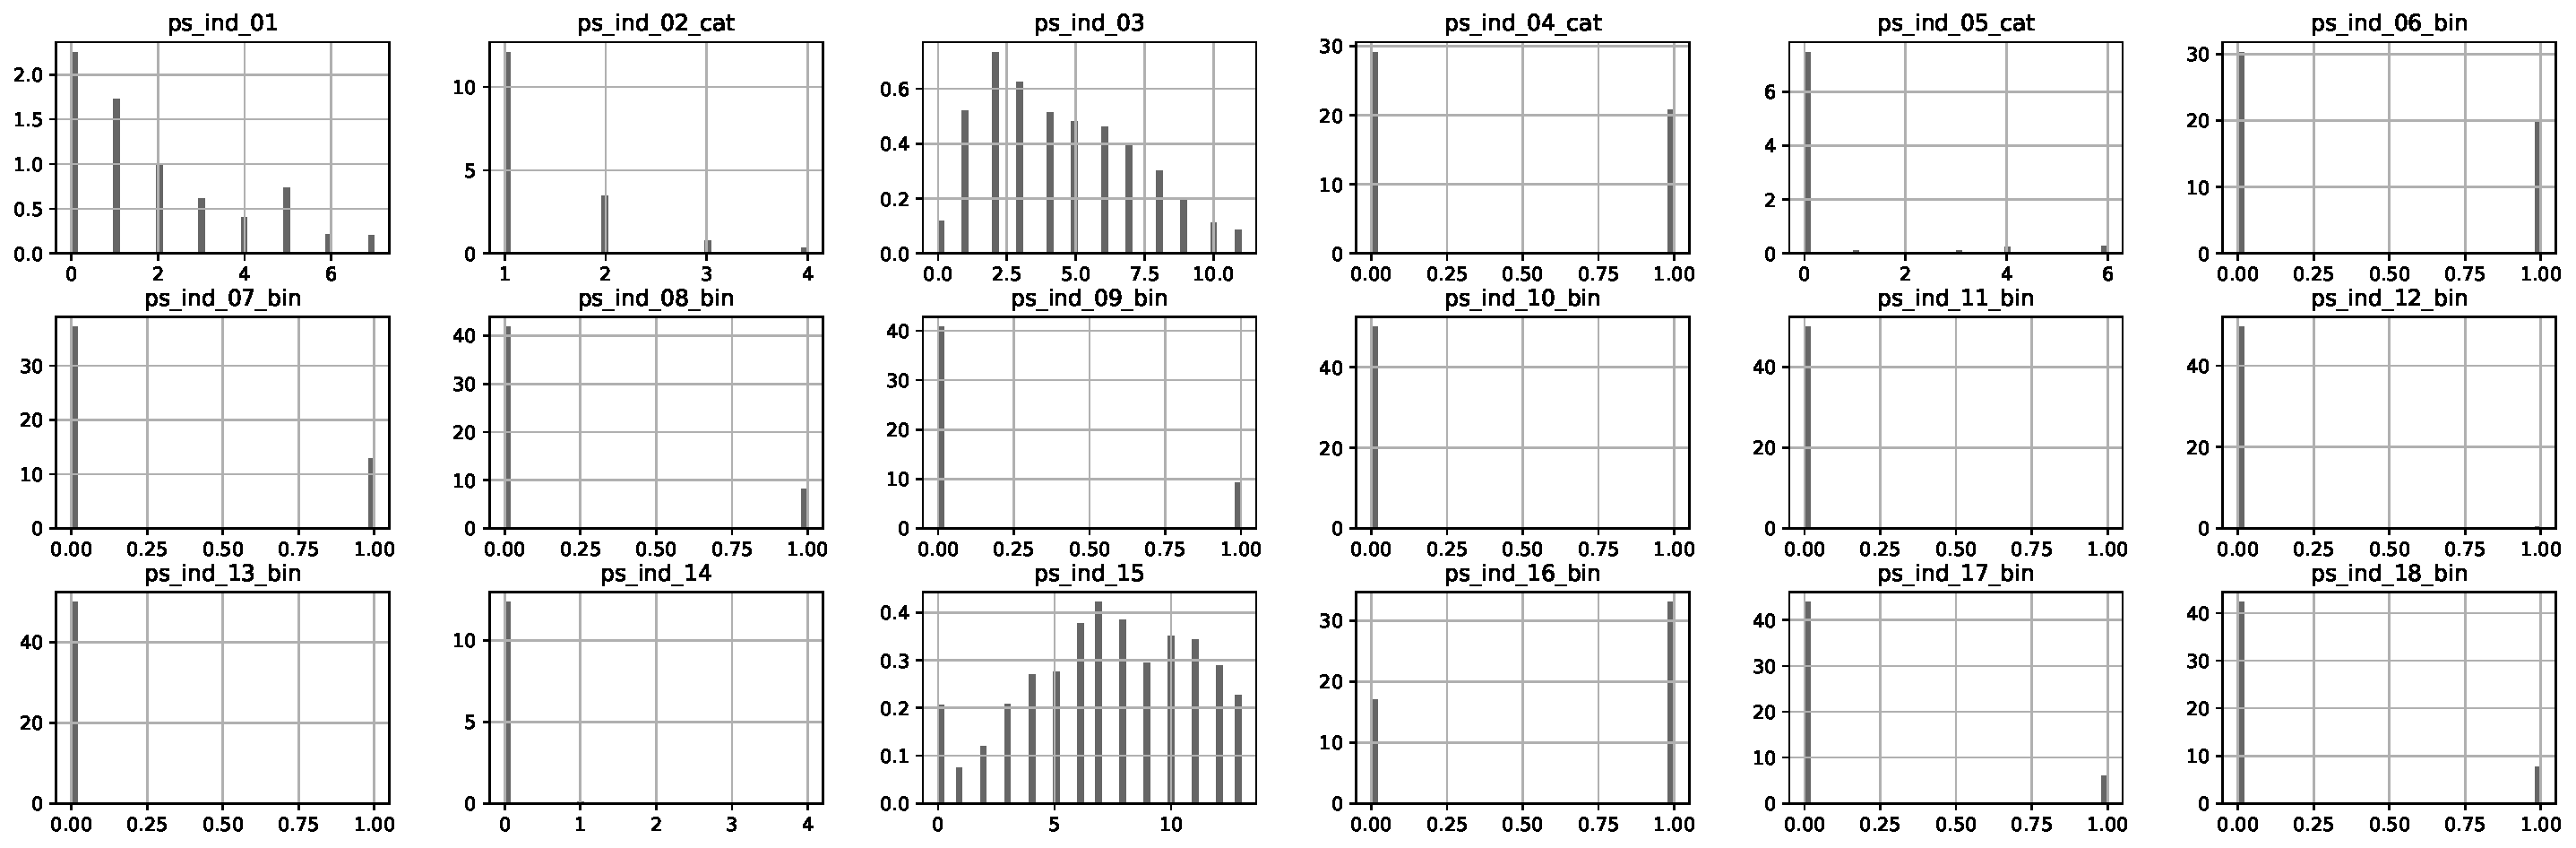
\includegraphics[width=\textwidth]{fig/ind_col.pdf}
\caption{Histogram for the \lstinline{ind} Attributes.}
\label{hist_ind}
\end{figure*}

\begin{figure}[!ht]
\centering
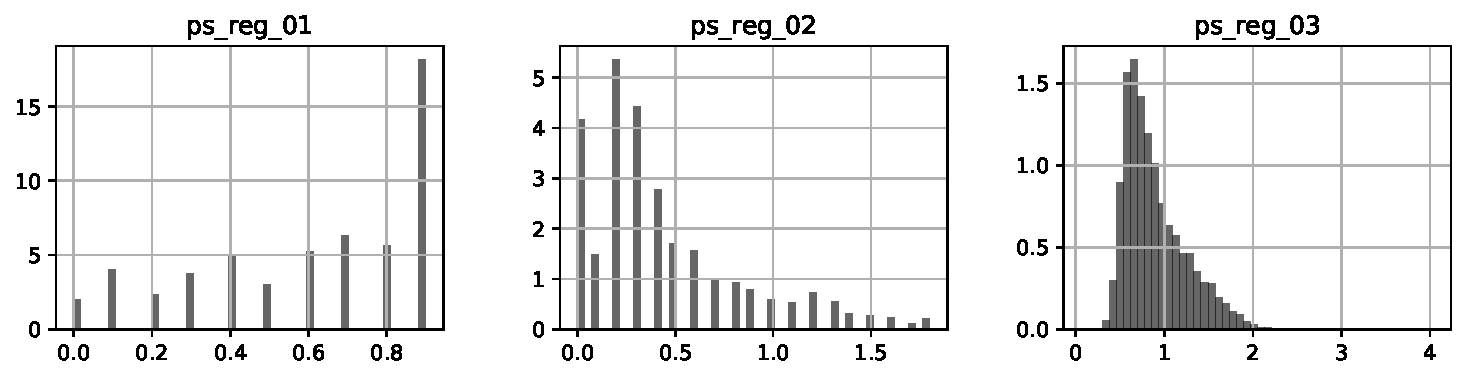
\includegraphics[width=.5\textwidth]{fig/reg_col.pdf}
\caption{Histogram for the \lstinline{reg} Attributes.}
\label{hist_reg}
\end{figure}

\begin{figure*}[!ht]
\centering
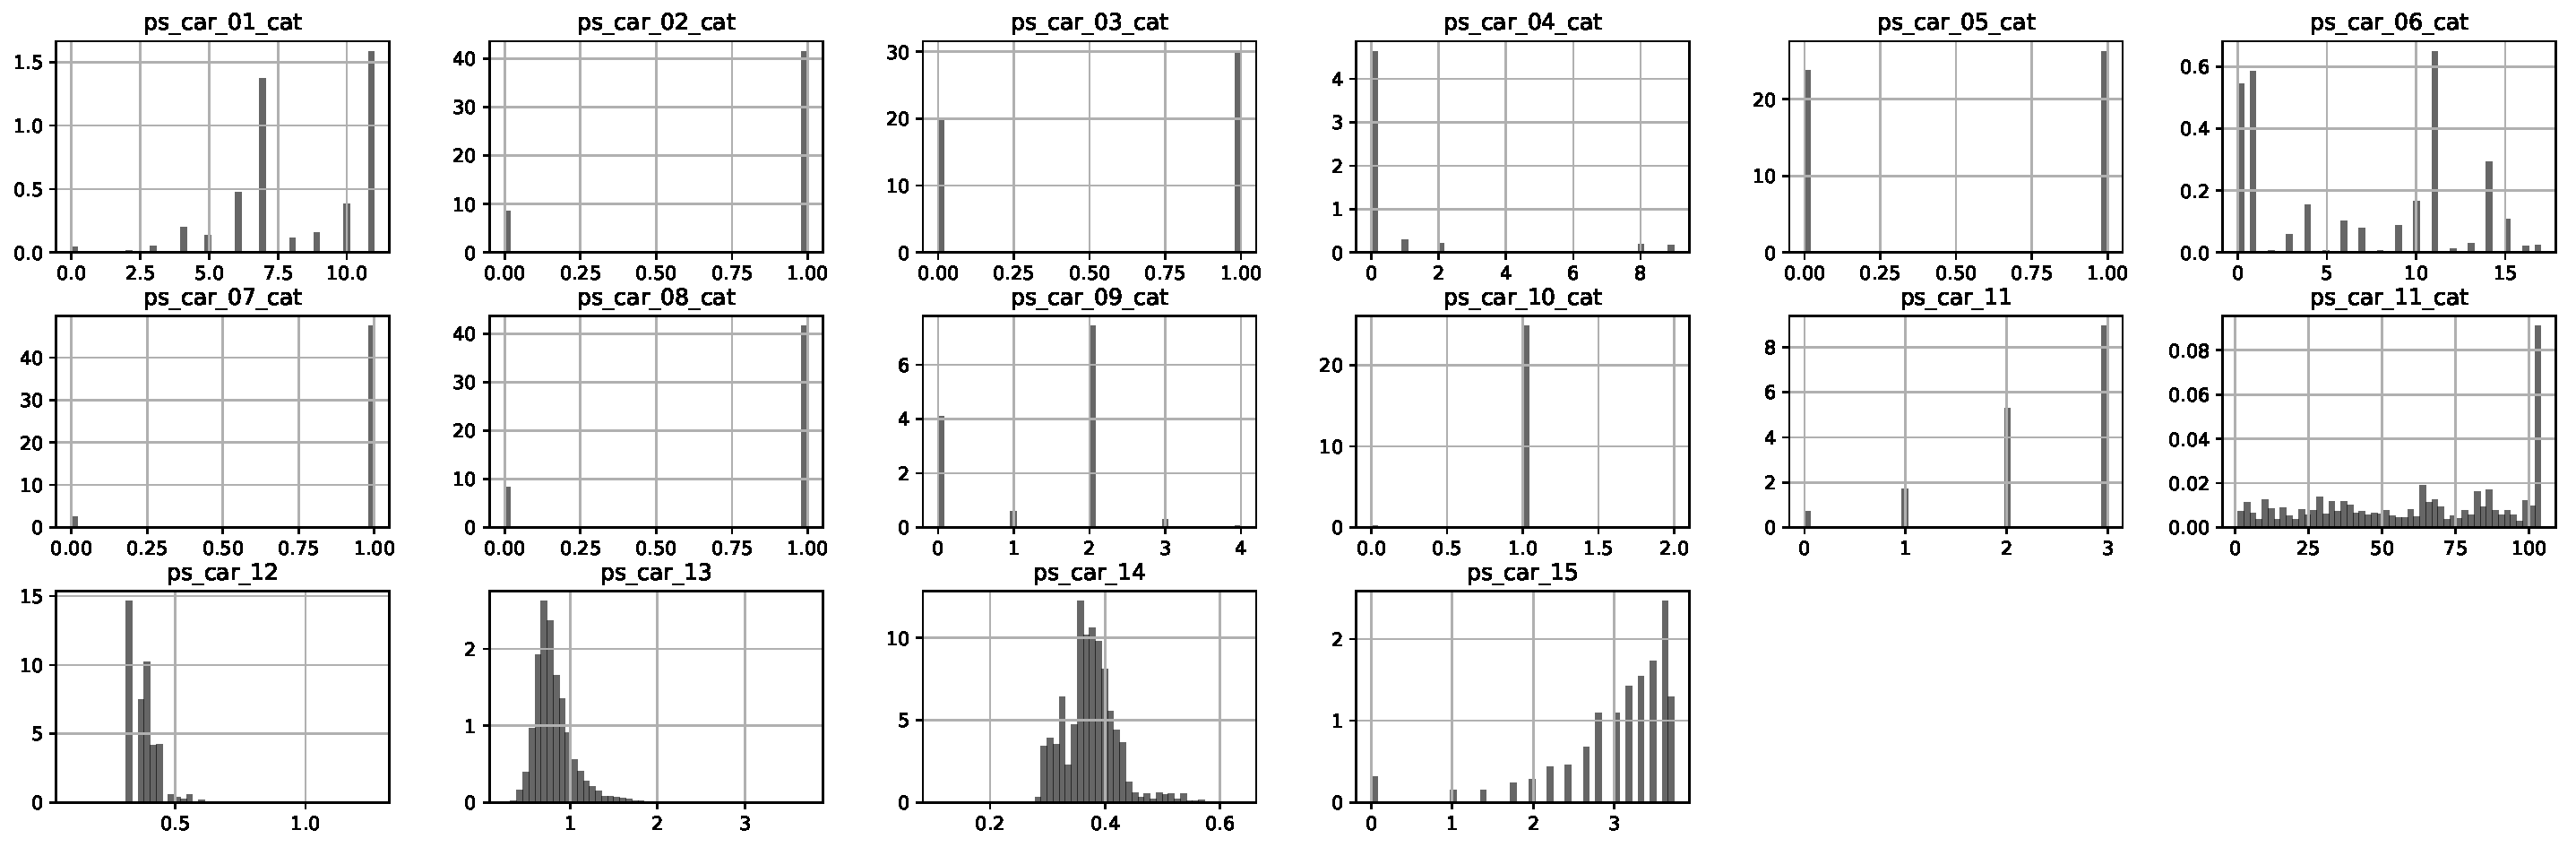
\includegraphics[width=\textwidth]{fig/car_col.pdf}
\caption{Histogram for the \lstinline{car} Attributes.}
\label{hist_car}
\end{figure*}

\begin{figure*}[!ht]
\centering
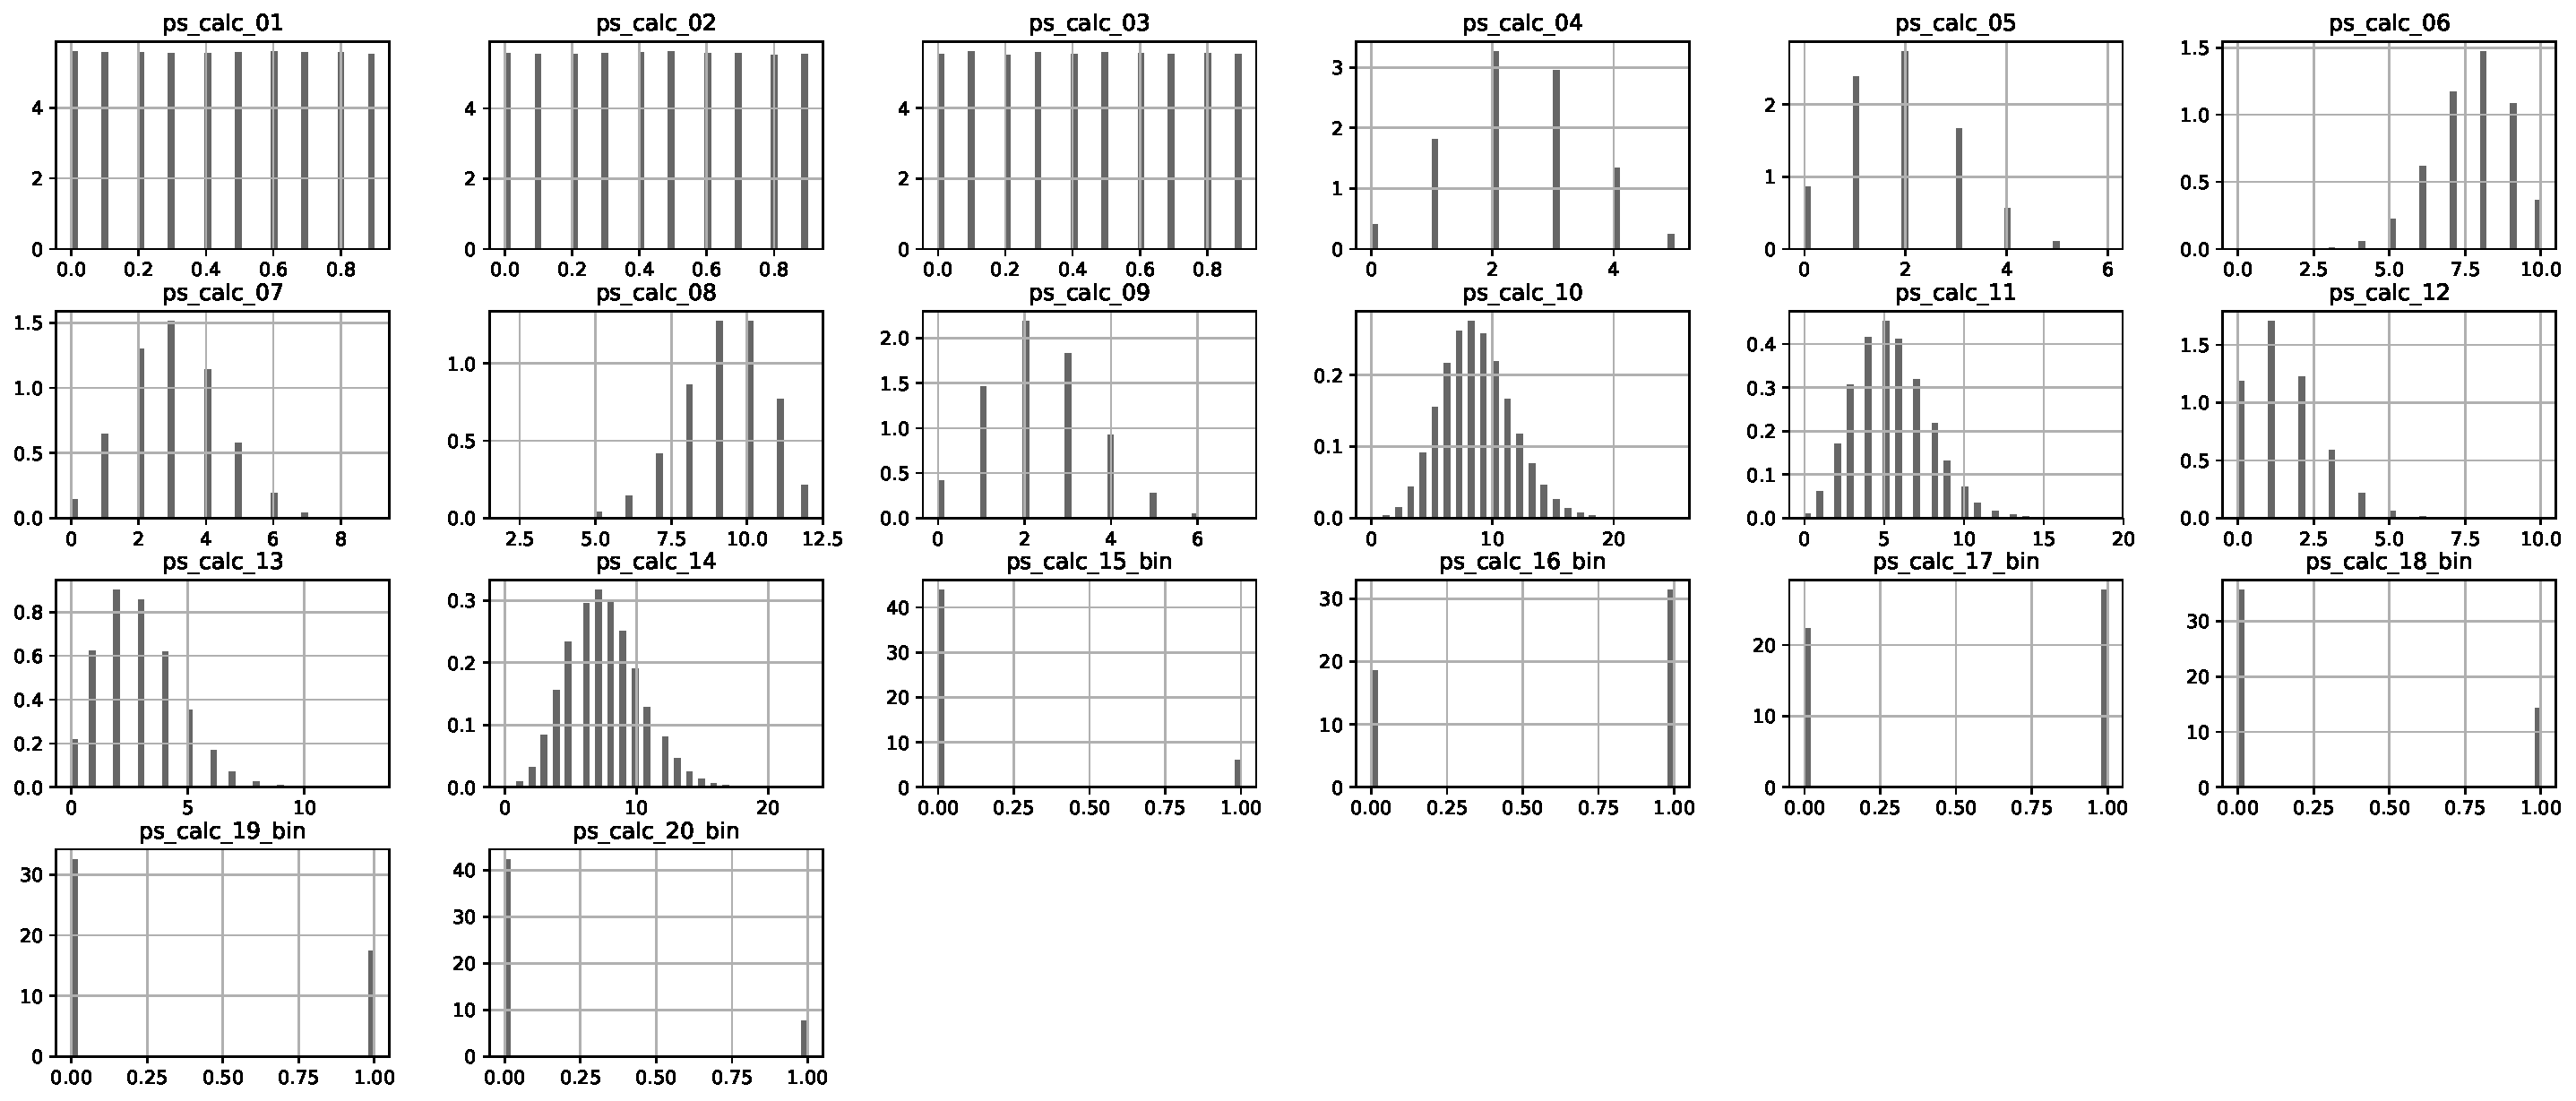
\includegraphics[width=\textwidth]{fig/calc_col.pdf}
\caption{Histogram for the \lstinline{calc} Attributes.}
\label{hist_calc}
\end{figure*}

From histograms, we may conclude the following:
\begin{itemize}
\item Some binary features are dominated by \lstinline{True} (\lstinline{False}), for example \lstinline{ps_ind_06-10}.
\item Some features' distribution are fairly even, for example \lstinline{ps_calc_01}, \lstinline{ps_calc_02} and \lstinline{ps_calc_03}.
\end{itemize}

It might seem plausible to discard these features in training phase. But the deletion requires more careful consideration. As mentioned above, \lstinline{ps_ind_06-10} might be \emph{one-hot encoded}, thus, all these four features would be naturally exclusive of each other.

\subsection{Correlation Analysis}

Features' Correlation within each category, i.e., \lstinline{ind}, \lstinline{reg}, \lstinline{car}, \lstinline{calc} are shown as histograms in appendix \cref{corr_ind}, \cref{corr_reg}, \cref{corr_car} and \cref{corr_calc} respectfully.



From correlation plot, we can conclude that strong correlation did not exist.
It it not possible to conduct any dimension reduction based on correlations
between features.

\subsection{Missing Value Mechanism and Data Imputation}

Values of -1 indicate that the feature was missing from
the observation. Missing values count in each feature is shown in \cref{missing_count}:

\begin{table}[!h]
\renewcommand{\arraystretch}{1.3}
\caption{Missing Value Counts in Each Feature}\label{missing_count}
\centering
\begin{tabular}{l|r|r}
\toprule
\bfseries Feature Name & \bfseries Count & \bfseries Percentage \\
\midrule
\verb|ps_ind_02_cat|  &      216 & 0.0363\%\\
\verb|ps_ind_04_cat|  &       83 & 0.0139\%\\
\verb|ps_ind_05_cat|  &     5809 & 0.9760\%\\
\verb|ps_reg_03|      &   107772 & 18.1065\%\\
\verb|ps_car_01_cat|  &      107 & 0.0180\%\\
\verb|ps_car_02_cat|  &        5 & 0.0008\%\\
\verb|ps_car_03_cat|  &   411231 & 69.0898\%\\
\verb|ps_car_05_cat|  &   266551 & 44.7825\%\\
\verb|ps_car_07_cat|  &    11489 & 1.9302\%\\
\verb|ps_car_09_cat|  &      569 & 0.0956\%\\
\verb|ps_car_11|      &        5 & 0.0008\%\\
\verb|ps_car_12|      &        1 & 0.0002\%\\
\verb|ps_car_14|      &    42620 & 7.1605\%\\
\bottomrule
\end{tabular}
\end{table}

There are several approaches to handle missing values\cite{Intro:Missing}:

\begin{itemize}
\item Deletion methods: cases with missing values are discarded, the analyses are restricted to cases that have
complete data.
\item Single imputation methods: imputes (i.e., \emph{fills in}) the missing data with seemingly suitable replacement values. Mean, median and mode are the most popular averaging techniques to use\cite{Missing:Howto}.
\item Multiple imputation methods: creates several copies of the data set, each containing different
imputed values. These method has greater performance but is harder to implemented.
\end{itemize}

From the table we can see that, most features have no missing value (only 13 features out of 51 have).
Some features only have a small amount of instances with missing value (\lstinline{ps_car_02_cat} and \lstinline{ps_car_11} have 5 missing value and \lstinline{ps_car_12} have only 1).

Based on these observation, we handled the missing values as follow:

\begin{itemize}
    \item For features with a few missing values, delete those data instances.
    \item For categorical features, we treat the missing values a new category.
    \item For numeric features, we use the mean of the population as missing value.
\end{itemize}

\end{document}


\documentclass{standalone}

\begin{document}

\section{Experimental Evaluation}

\subsection{Methodology}

% \scriptsize{
% What are criteria you are using to evaluate your method? What specific
% hypotheses does your experiment test? Describe the experimental methodology
% that you used. What are the dependent and independent variables? What is the
% training/test data that was used, and why is it realistic or interesting?
% Exactly what performance data did you collect and how are you presenting and
% analyzing it? Comparisons to competing methods that address the same problem
% are particularly useful. 
% }\normalsize

We used per-class accuracy, AUC and Normalized Gini Coefficient to evaluate out model.

\subsubsection{Per-Class Accuracy}

Accuracy simply measures how often the classifier makes the correct prediction. It’s the ratio between the number of correct predictions and the total number of predictions (the number of data points in the test set)\cite{Alice:2015:Evaluating}:
\begin{IEEEeqnarray}{C} 
accuracy = \frac{\mathrm{\#\ correct\ predictions}}{\mathrm{\#\ total\ data\ points}}\IEEEnonumber
\end{IEEEeqnarray}

Per-class accuracy is the average of the accuracy for each class. By using per-class accuracy, we can have a better understanding of the model if the target class was dominated by one label.

\subsubsection{Normalized Gini Coefficient and AUC}

The Normalized Gini coefficient, (named for the similar Gini coefficient/index used in Economics, which originally developed by Italian statistician and sociologist Corrado Gini\cite{Gini:1912}), measures the inequality among values of a frequency distribution (for example, levels of income)\cite{Gini:Wikipedia}. It is most commonly defined as twice the area between the ROC curve and the diagonal (with this area being taken as negative in the rare event that the curve lies below the diagonal).

AUC stands for area under the curve.

The normalized Gini coefficient and AUC are closely related. When using normalized units, the AUC is equal to the probability that a classifier will rank a randomly chosen positive instance higher than a randomly chosen negative one (assuming 'positive' ranks higher than 'negative')\cite{Fawcett:2006:IRA:1159473.1159475}. Elementary geometry shows that 
\begin{IEEEeqnarray}{C} 
Gini = 2 \times \mathrm{AUC} - 1.
\end{IEEEeqnarray}

The competition used normalized Gini coefficient to measure participants' submission performance. In our experiment, we worked in terms of AUC, but the results apply equally to the Gini coefficient.

% \subsection{Results}

% \scriptsize{
% Present the quantitative results of your experiments. Graphical data
% presentation such as graphs and histograms are frequently better than tables.
% What are the basic differences revealed in the data. Are they statistically
% significant? 
% }\normalsize

% \subsection{Discussion}

% \scriptsize{
% Is your hypothesis supported? What conclusions do the results support about the
% strengths and weaknesses of your method compared to other methods? How can the
% results be explained in terms of the underlying properties of the algorithm
% and/or the data. 
% }\normalsize

\end{document}

\section{Coding Language}

The main coding language is \emph{Python 3.x} with following machine learning library:
\begin{itemize}
    \item pandas.
    \item scikit-learn.
    \item tensorflow.
\end{itemize}

% \section{Related Work}

% \scriptsize{
% Answer the following questions for each piece of related work that addresses
% the same or a similar problem. What is their problem and method? How is your
% problem and method different? Why is your problem and method better? 
% }\normalsize

% \section{Future Work}

% \scriptsize{
% What are the major shortcomings of your current method? For each shortcoming,
% propose additions or enhancements that would help overcome it. 
% }\normalsize

% \section{Conclusion}

% \scriptsize{
% Briefly summarize the important results and conclusions presented in the paper.
% What are the most important points illustrated by your work? How will your
% results improve future research and applications in the area? 
% }\normalsize

% \section{Bilbiography}

% \scriptsize{
% Be sure to include a standard, well-formated, comprehensive bibliography with
% citations from the text referring to previously published papers in the
% scientific literature that you utilized or are related to your work.
% }\normalsize

% \lipsum[3-10]

\bibliography{report.bib}{}
\bibliographystyle{plain}

\end{document}
